% --- LaTeX Lecture Notes Template - S. Venkatraman ---

% --- Set document class and font size ---

\documentclass[letterpaper, 12pt]{article}


% --- Package imports ---

% Extended set of colors
\usepackage[dvipsnames]{xcolor}

\usepackage{
  amsmath, amsthm, amssymb, mathtools, dsfont, units,          % Math typesetting
  graphicx, wrapfig, subfig, float,                            % Figures and graphics formatting
  listings, color, inconsolata, pythonhighlight,               % Code formatting
  fancyhdr, sectsty, hyperref, enumerate, enumitem, framed }   % Headers/footers, section fonts, links, lists

% lipsum is just for generating placeholder text and can be removed
\usepackage{hyperref, lipsum} 
% \usepackage{bm}
% \usepackage{subfig}

% --- Fonts ---

\usepackage{newpxtext, newpxmath, inconsolata}
\usepackage{amsfonts}
\usepackage{pgfplots}
\pgfplotsset{compat=1.12}
\usepackage{tkz-fct}
\usepackage{svg}
\usepackage{tikz}
\usepackage{tikz-cd}
\usepackage{lipsum}
\usepackage{enumitem}
\usepackage[title]{appendix}
% \usepackage[toc,page]{appxendix}
\usepackage[utf8]{inputenc}
\usepackage{multicol}
\usepackage{multirow}
\usepackage{booktabs}

\usepackage{minted}  % code highlighting
% \usepackage[finalizecache,cachedir=.]{minted}
% \usepackage[frozencache,cachedir=.]{minted}

\DeclareUnicodeCharacter{3BC}{$\pi$}
\DeclareUnicodeCharacter{3C0}{$\pi$}

\usepackage[most]{tcolorbox}
\newtcolorbox{myquote}[1][]{%
  colback=black!5,
  colframe=black!5,
  notitle,
  sharp corners,
  % borderline west={2pt}{0pt}{red!80!black},
  enhanced,
  breakable,
}

\renewcommand*\pod[1]{%
  \allowbreak
  \mathchoice
    {\mkern 18mu}%
    {\mkern  8mu}%
    {\mkern  6mu}% "6mu" matches the space *after* the word "mod"
    {\mkern  6mu}%
  (#1)%
}

% --- Page layout settings ---

% Set page margins
\usepackage[left=1.35in, right=1.35in, top=1.0in, bottom=.9in, headsep=.2in, footskip=0.35in]{geometry}

% Anchor footnotes to the bottom of the page
\usepackage[bottom]{footmisc}

% Set line spacing
\renewcommand{\baselinestretch}{1.2}

% Set spacing between paragraphs
\setlength{\parskip}{1.3mm}

% Allow multi-line equations to break onto the next page
\allowdisplaybreaks

% --- Page formatting settings ---

% Set image captions to be italicized
\usepackage[font={it,footnotesize}]{caption}

% Set link colors for labeled items (blue), citations (red), URLs (orange)
\hypersetup{colorlinks=true, linkcolor=RoyalBlue, citecolor=RedOrange, urlcolor=ForestGreen}

% Set font size for section titles (\large) and subtitles (\normalsize) 
\usepackage{titlesec}
% \titleformat{\section}{\large\bfseries}{{\fontsize{19}{19}\selectfont\textreferencemark}\;\; }{0em}{}
\titleformat{\section}{\large\bfseries}{\thesection\;\;\;}{0em}{}
\titleformat{\subsection}{\normalsize\bfseries\selectfont}{\thesubsection\;\;\;}{0em}{}

% Enumerated/bulleted lists: make numbers/bullets flush left
%\setlist[enumerate]{wide=2pt, leftmargin=16pt, labelwidth=0pt}
\setlist[itemize]{wide=0pt, leftmargin=16pt, labelwidth=10pt, align=left}

% --- Table of contents settings ---

\usepackage[subfigure]{tocloft}

% Reduce spacing between sections in table of contents
\setlength{\cftbeforesecskip}{.9ex}

% Remove indentation for sections
\cftsetindents{section}{0em}{0em}

% Set font size (\large) for table of contents title
\renewcommand{\cfttoctitlefont}{\large\bfseries}

% Remove numbers/bullets from section titles in table of contents
\makeatletter
\renewcommand{\cftsecpresnum}{\begin{lrbox}{\@tempboxa}}
\renewcommand{\cftsecaftersnum}{\end{lrbox}}
\makeatother

% --- Set path for images ---

\graphicspath{{Images/}{../Images/}}

% --- Math/Statistics commands ---

% Add a reference number to a single line of a multi-line equation
% Usage: "\numberthis\label{labelNameHere}" in an align or gather environment
\newcommand\numberthis{\addtocounter{equation}{1}\tag{\theequation}}

% Shortcut for bold text in math mode, e.g. $\b{X}$
\let\b\mathbf

% Shortcut for bold Greek letters, e.g. $\bg{\beta}$
\let\bg\boldsymbol

% Shortcut for calligraphic script, e.g. %\mc{M}$
\let\mc\mathcal

% \mathscr{(letter here)} is sometimes used to denote vector spaces
\usepackage[mathscr]{euscript}

% Convergence: right arrow with optional text on top
% E.g. $\converge[p]$ for converges in probability
\newcommand{\converge}[1][]{\xrightarrow{#1}}

% Weak convergence: harpoon symbol with optional text on top
% E.g. $\wconverge[n\to\infty]$
\newcommand{\wconverge}[1][]{\stackrel{#1}{\rightharpoonup}}

% Equality: equals sign with optional text on top
% E.g. $X \equals[d] Y$ for equality in distribution
\newcommand{\equals}[1][]{\stackrel{\smash{#1}}{=}}

% Normal distribution: arguments are the mean and variance
% E.g. $\normal{\mu}{\sigma}$
\newcommand{\normal}[2]{\mathcal{N}\left(#1,#2\right)}

% Uniform distribution: arguments are the left and right endpoints
% E.g. $\unif{0}{1}$
\newcommand{\unif}[2]{\text{Uniform}(#1,#2)}

% Independent and identically distributed random variables
% E.g. $ X_1,...,X_n \iid \normal{0}{1}$
\newcommand{\iid}{\stackrel{\smash{\text{iid}}}{\sim}}

% Sequences (this shortcut is mostly to reduce finger strain for small hands)
% E.g. to write $\{A_n\}_{n\geq 1}$, do $\bk{A_n}{n\geq 1}$
\newcommand{\bk}[2]{\{#1\}_{#2}}

\newcommand{\what}[1]{\widehat{#1}}
% \setcounter{section}{-1}

\setcounter{MaxMatrixCols}{20}

\newcommand{\SL}{\mathrm{SL}}
\newcommand{\Sp}{\mathrm{Sp}}
\newcommand{\Mp}{\mathrm{Mp}}
\newcommand{\GL}{\mathrm{GL}}
\newcommand{\SO}{\mathrm{SO}}
\newcommand{\SU}{\mathrm{SU}}
\newcommand{\PGL}{\mathrm{PGL}}
\newcommand{\PSL}{\mathrm{PSL}}
\newcommand{\GSp}{\mathrm{GSp}}
\newcommand{\PGSp}{\mathrm{PGSp}}
\newcommand{\Spin}{\mathrm{Spin}}
\newcommand{\gl}{\mathfrak{gl}}
\newcommand{\JL}{\mathrm{JL}}
\newcommand{\stab}{\mathrm{Stab}}
% \newcommand{\ab}{\mathrm{ab}}
\newcommand{\cha}{\mathrm{char}}
\newcommand{\fin}{\mathrm{fin}}
\newcommand{\Tr}{\mathrm{Tr}}
\newcommand{\Li}{\mathrm{Li}}
\newcommand{\trdeg}{\mathrm{trdeg}}
\newcommand{\rank}{\mathrm{rank}}
\newcommand{\rad}{\mathrm{rad}}
\newcommand{\Res}{\mathrm{Res}}
\newcommand{\Hom}{\mathrm{Hom}}
\newcommand{\Spec}{\mathrm{Spec}\,}
\newcommand{\Sym}{\mathrm{Sym}}
\newcommand{\ev}{\mathrm{ev}}
\newcommand{\disc}{\mathrm{disc}}
\newcommand{\Aut}{\mathrm{Aut}}
\newcommand{\Span}{\mathrm{Span}}
\newcommand{\supp}{\mathrm{supp}}
\newcommand{\sgn}{\mathrm{sgn}}
\newcommand{\Lie}{\mathrm{Lie}}
\newcommand{\Ind}{\mathrm{Ind}}
\newcommand{\pInd}{\mathrm{pInd}}
\newcommand{\Gal}{\mathrm{Gal}}
\newcommand{\Cl}{\mathrm{Cl}}
\newcommand{\Wh}{\mathrm{Wh}}
\newcommand{\std}{\mathrm{std}}
\newcommand{\Slit}{\mathrm{Slit}}
\newcommand{\pprod}{\sideset{}{'}\prod}
\newcommand{\potimes}{\sideset{}{'}\otimes}
\newcommand{\pbigotimes}{\sideset{}{'}\bigotimes}
% \sideset{}{'}\prod
\newcommand{\RQM}{\mathcal{RQM}}

\newcommand{\QM}{\mathcal{QM}}

\newcommand{\dd}{\mathrm{d}}
\newcommand{\dso}{\mathds{1}}

\newcommand{\llb}{\llbracket}
\newcommand{\rrb}{\rrbracket}

\newcommand{\rA}{\mathrm{A}}
\newcommand{\rB}{\mathrm{B}}
\newcommand{\rC}{\mathrm{C}}
\newcommand{\rD}{\mathrm{D}}
\newcommand{\rE}{\mathrm{E}}
\newcommand{\rF}{\mathrm{F}}
\newcommand{\rG}{\mathrm{G}}
\newcommand{\rH}{\mathrm{H}}
\newcommand{\rI}{\mathrm{I}}
\newcommand{\rJ}{\mathrm{J}}
\newcommand{\rK}{\mathrm{K}}
\newcommand{\rL}{\mathrm{L}}
\newcommand{\rM}{\mathrm{M}}
\newcommand{\rN}{\mathrm{N}}
\newcommand{\rO}{\mathrm{O}}
\newcommand{\rP}{\mathrm{P}}
\newcommand{\rQ}{\mathrm{Q}}
\newcommand{\rR}{\mathrm{R}}
\newcommand{\rS}{\mathrm{S}}
\newcommand{\rT}{\mathrm{T}}
\newcommand{\rU}{\mathrm{U}}
\newcommand{\rV}{\mathrm{V}}
\newcommand{\rW}{\mathrm{W}}
\newcommand{\rX}{\mathrm{X}}
\newcommand{\rY}{\mathrm{Y}}
\newcommand{\rZ}{\mathrm{Z}}

\newcommand{\bA}{\mathbb{A}}
\newcommand{\bB}{\mathbb{B}}
\newcommand{\bC}{\mathbb{C}}
\newcommand{\bD}{\mathbb{D}}
\newcommand{\bE}{\mathbb{E}}
\newcommand{\bF}{\mathbb{F}}
\newcommand{\bG}{\mathbb{G}}
\newcommand{\bH}{\mathbb{H}}
\newcommand{\bI}{\mathbb{I}}
\newcommand{\bJ}{\mathbb{J}}
\newcommand{\bK}{\mathbb{K}}
\newcommand{\bL}{\mathbb{L}}
\newcommand{\bM}{\mathbb{M}}
\newcommand{\bN}{\mathbb{N}}
\newcommand{\bO}{\mathbb{O}}
\newcommand{\bP}{\mathbb{P}}
\newcommand{\bQ}{\mathbb{Q}}
\newcommand{\bR}{\mathbb{R}}
\newcommand{\bS}{\mathbb{S}}
\newcommand{\bT}{\mathbb{T}}
\newcommand{\bU}{\mathbb{U}}
\newcommand{\bV}{\mathbb{V}}
\newcommand{\bW}{\mathbb{W}}
\newcommand{\bX}{\mathbb{X}}
\newcommand{\bY}{\mathbb{Y}}
\newcommand{\bZ}{\mathbb{Z}}

\newcommand{\bx}{\mathbf{x}}
\newcommand{\by}{\mathbf{y}}

\newcommand{\cA}{\mathcal{A}}
\newcommand{\cB}{\mathcal{B}}
\newcommand{\cC}{\mathcal{C}}
\newcommand{\cD}{\mathcal{D}}
\newcommand{\cE}{\mathcal{E}}
\newcommand{\cF}{\mathcal{F}}
\newcommand{\cG}{\mathcal{G}}
\newcommand{\cH}{\mathcal{H}}
\newcommand{\cI}{\mathcal{I}}
\newcommand{\cJ}{\mathcal{J}}
\newcommand{\cK}{\mathcal{K}}
\newcommand{\cL}{\mathcal{L}}
\newcommand{\cM}{\mathcal{M}}
\newcommand{\cN}{\mathcal{N}}
\newcommand{\cO}{\mathcal{O}}
\newcommand{\cP}{\mathcal{P}}
\newcommand{\cQ}{\mathcal{Q}}
\newcommand{\cR}{\mathcal{R}}
\newcommand{\cS}{\mathcal{S}}
\newcommand{\cT}{\mathcal{T}}
\newcommand{\cU}{\mathcal{U}}
\newcommand{\cV}{\mathcal{V}}
\newcommand{\cW}{\mathcal{W}}
\newcommand{\cX}{\mathcal{X}}
\newcommand{\cY}{\mathcal{Y}}
\newcommand{\cZ}{\mathcal{Z}}

\newcommand{\scA}{\mathscr{A}}
\newcommand{\scB}{\mathscr{B}}
\newcommand{\scC}{\mathscr{C}}
\newcommand{\scD}{\mathscr{D}}
\newcommand{\scE}{\mathscr{E}}
\newcommand{\scF}{\mathscr{F}}
\newcommand{\scG}{\mathscr{G}}
\newcommand{\scH}{\mathscr{H}}
\newcommand{\scI}{\mathscr{I}}
\newcommand{\scJ}{\mathscr{J}}
\newcommand{\scK}{\mathscr{K}}
\newcommand{\scL}{\mathscr{L}}
\newcommand{\scM}{\mathscr{M}}
\newcommand{\scN}{\mathscr{N}}
\newcommand{\scO}{\mathscr{O}}
\newcommand{\scP}{\mathscr{P}}
\newcommand{\scQ}{\mathscr{Q}}
\newcommand{\scR}{\mathscr{R}}
\newcommand{\scS}{\mathscr{S}}
\newcommand{\scT}{\mathscr{T}}
\newcommand{\scU}{\mathscr{U}}
\newcommand{\scV}{\mathscr{V}}
\newcommand{\scW}{\mathscr{W}}
\newcommand{\scX}{\mathscr{X}}
\newcommand{\scY}{\mathscr{Y}}
\newcommand{\scZ}{\mathscr{Z}}

\newcommand{\frA}{\mathfrak{A}}
\newcommand{\frB}{\mathfrak{B}}
\newcommand{\frC}{\mathfrak{C}}
\newcommand{\frD}{\mathfrak{D}}
\newcommand{\frE}{\mathfrak{E}}
\newcommand{\frF}{\mathfrak{F}}
\newcommand{\frG}{\mathfrak{G}}
\newcommand{\frH}{\mathfrak{H}}
\newcommand{\frI}{\mathfrak{I}}
\newcommand{\frJ}{\mathfrak{J}}
\newcommand{\frK}{\mathfrak{K}}
\newcommand{\frL}{\mathfrak{L}}
\newcommand{\frM}{\mathfrak{M}}
\newcommand{\frN}{\mathfrak{N}}
\newcommand{\frO}{\mathfrak{O}}
\newcommand{\frP}{\mathfrak{P}}
\newcommand{\frQ}{\mathfrak{Q}}
\newcommand{\frR}{\mathfrak{R}}
\newcommand{\frS}{\mathfrak{S}}
\newcommand{\frT}{\mathfrak{T}}
\newcommand{\frU}{\mathfrak{U}}
\newcommand{\frV}{\mathfrak{V}}
\newcommand{\frW}{\mathfrak{W}}
\newcommand{\frX}{\mathfrak{X}}
\newcommand{\frY}{\mathfrak{Y}}
\newcommand{\frZ}{\mathfrak{Z}}

\newcommand{\fra}{\mathfrak{a}}
\newcommand{\frb}{\mathfrak{b}}
\newcommand{\frc}{\mathfrak{c}}
\newcommand{\frd}{\mathfrak{d}}
\newcommand{\fre}{\mathfrak{e}}
\newcommand{\frf}{\mathfrak{f}}
\newcommand{\frg}{\mathfrak{g}}
\newcommand{\frh}{\mathfrak{h}}
\newcommand{\fri}{\mathfrak{i}}
\newcommand{\frj}{\mathfrak{j}}
\newcommand{\frk}{\mathfrak{k}}
\newcommand{\frl}{\mathfrak{l}}
\newcommand{\frm}{\mathfrak{m}}
\newcommand{\frn}{\mathfrak{n}}
\newcommand{\fro}{\mathfrak{o}}
\newcommand{\frp}{\mathfrak{p}}
\newcommand{\frq}{\mathfrak{q}}
\newcommand{\frr}{\mathfrak{r}}
\newcommand{\frs}{\mathfrak{s}}
\newcommand{\frt}{\mathfrak{t}}
\newcommand{\fru}{\mathfrak{u}}
\newcommand{\frv}{\mathfrak{v}}
\newcommand{\frw}{\mathfrak{w}}
\newcommand{\frx}{\mathfrak{x}}
\newcommand{\fry}{\mathfrak{y}}
\newcommand{\frz}{\mathfrak{z}}

\newcommand{\sage}{\raisebox{-0.16\height}{
\includegraphics[height=1em]{./sagelogo.png}}\,\,}

% Math mode symbols for common sets and spaces. Example usage: $\R$
\newcommand{\R}{\mathbb{R}}	% Real numbers
\newcommand{\C}{\mathbb{C}}	% Complex numbers
\newcommand{\Q}{\mathbb{Q}}	% Rational numbers
\newcommand{\Z}{\mathbb{Z}}	% Integers
\newcommand{\N}{\mathbb{N}}	% Natural numbers
\newcommand{\F}{\mathcal{F}}	% Calligraphic F for a sigma algebra
\newcommand{\El}{\mathcal{L}}	% Calligraphic L, e.g. for L^p spaces

% Math mode symbols for probability
\newcommand{\pr}{\mathbb{P}}	% Probability measure
\newcommand{\E}{\mathbb{E}}	% Expectation, e.g. $\E(X)$
\newcommand{\var}{\text{Var}}	% Variance, e.g. $\var(X)$
\newcommand{\cov}{\text{Cov}}	% Covariance, e.g. $\cov(X,Y)$
\newcommand{\corr}{\text{Corr}}	% Correlation, e.g. $\corr(X,Y)$
\newcommand{\B}{\mathcal{B}}	% Borel sigma-algebra

% Other miscellaneous symbols
\newcommand{\tth}{\text{th}}	% Non-italicized 'th', e.g. $n^\tth$
\newcommand{\Oh}{\mathcal{O}}	% Big-O notation, e.g. $\O(n)$
\newcommand{\1}{\mathds{1}}	% Indicator function, e.g. $\1_A$

\newcommand{\nul}{\mathrm{null}}
\newcommand{\range}{\mathrm{range}}

% Additional commands for math mode
\newcommand*{\argmax}{argmax}		% Argmax, e.g. $\argmax_{x\in[0,1]} f(x)$
\newcommand*{\argmin}{argmin}		% Argmin, e.g. $\argmin_{x\in[0,1]} f(x)$
\newcommand*{\spann}{Span}		% Span, e.g. $\spann\{X_1,...,X_n\}$
\newcommand*{\bias}{Bias}		% Bias, e.g. $\bias(\hat\theta)$
\newcommand*{\ran}{ran}			% Range of an operator, e.g. $\ran(T) 
\newcommand*{\dv}{d\!}			% Non-italicized 'with respect to', e.g. $\int f(x) \dv x$
\newcommand*{\diag}{diag}		% Diagonal of a matrix, e.g. $\diag(M)$
\newcommand*{\trace}{Tr}		% Trace of a matrix, e.g. $\trace(M)$
% \newcommand*{\supp}{supp}		% Support of a function, e.g., $\supp(f)$

% Numbered theorem, lemma, etc. settings - e.g., a definition, lemma, and theorem appearing in that 
% order in Lecture 2 will be numbered Definition 2.1, Lemma 2.2, Theorem 2.3. 
% Example usage: \begin{theorem}[Name of theorem] Theorem statement \end{theorem}
\theoremstyle{definition}
\newtheorem{theorem}{Theorem}[section]
\newtheorem{proposition}[theorem]{Proposition}
\newtheorem{lemma}[theorem]{Lemma}
\newtheorem{corollary}[theorem]{Corollary}
\newtheorem{definition}[theorem]{Definition}
\newtheorem{example}[theorem]{Example}
\newtheorem{question}[theorem]{Question}
\newtheorem{conjecture}[theorem]{Conjecture}
\newtheorem{exercise}[subsubsection]{Exercise}

\theoremstyle{remark}
\newtheorem{remark}[theorem]{Remark}

% Un-numbered theorem, lemma, etc. settings
% Example usage: \begin{lemma*}[Name of lemma] Lemma statement \end{lemma*}
\newtheorem*{theorem*}{Theorem}
\newtheorem*{proposition*}{Proposition}
\newtheorem*{lemma*}{Lemma}
\newtheorem*{corollary*}{Corollary}
\newtheorem*{definition*}{Definition}
\newtheorem*{example*}{Example}
\newtheorem*{remark*}{Remark}
\newtheorem*{claim}{Claim}
\newtheorem*{conjecture*}{Conjecture}

% --- Left/right header text (to appear on every page) ---

% Do not include a line under header or above footer
\pagestyle{fancy}
\renewcommand{\footrulewidth}{0pt}
\renewcommand{\headrulewidth}{0pt}

% Right header text: Lecture number and title
\renewcommand{\sectionmark}[1]{\markright{#1} }
% \fancyhead[R]{\small\textit{\nouppercase{\rightmark}}}

% Left header text: Short course title, hyperlinked to table of contents
% \fancyhead[L]{\hyperref[sec:contents]{\small Matrix multplication}}

% \pgfkeys{/Dynkin diagram,
% edge length=1.5cm,
% fold radius=1cm,
% indefinite edge/.style={
% draw=black,
% fill=white,
% thin,
% densely dashed}}

\usepackage{fancyhdr}
\pagestyle{fancy}
\fancyhead[R]{}
\fancyhead[L]{}

% --- Document starts here ---

\begin{document}

% --- Main title and subtitle ---

\title{Singular Algebraic Curves}
% \\[1em]
% \normalsize Re-typed by Seewoo Lee\footnote{seewoo5@berkeley.edu}}

% --- Author and date of last update ---

\author{Seewoo Lee}
% \date{\normalsize\vspace{-1ex} Last updated: \today}
\date{}

% --- Add title and table of contents ---

\maketitle


% --- Abstracts ---

This note closely follows Chapter 4 of Serre's \emph{Algebraic Groups and Class Fields}.
We generalize the theory in Chapter 2 to \emph{nonsingular} curves via normalization.
We also associate a singular curve $X_\frm$ to a modulus $\frm$ of a nonsingular curve $X$, which will be used in the construction of generalized Jacobians later.
Most of the theorems (Riemann--Roch, Serre duality) hold when we replace $\cL(D)$ and $\underline{\Omega}(D)$ with appropriate notions $\cL'(D)$ and $\underline{\Omega}'(D)$ for singular curves, and the genus $g$ with \emph{arithmetic} genus.

% \tableofcontents\label{sec:contents}

% --- Main content: import lectures as subfiles ---

\section{Structure of a singular algebraic curve}

\subsection{Normalization of an algebraic variety}

For an irreducible algebraic variety $X'$, \emph{normalization} $X \to X'$ can be constructed locally as taking integral closure $\scO_Q$ of each $\scO'_Q$ in $K = k(X')$.
For an affine open $U' \subset X'$ with $A' = \scO'(U')$, the corresponding normal affine variety $U \to U'$ corresponds to an integral closure $A$ of $A'$ in $K$, and \emph{glueing} these $U$ give $X$.
Let $\scO = p_\ast(\scO_X)$, whose stalks are $\scO_Q = \cap_{P\to Q} \scO_P$ and $\scO'$ is a subsheaf of $\scO$.
See \href{https://mathoverflow.net/questions/109395/is-there-a-geometric-intuition-underlying-the-notion-of-normal-varieties}{this MO answer} for the nice geometric intuitions of normal varieties.

Here's an example from \href{https://math.stanford.edu/~vakil/725/class20.pdf}{Vakil's note}: consider a \emph{nodal curve} $X': y^2 = x^3 + x^2$, singularity at $(0,0)$.
One needs to normalize the ring $R = k[x, y] / (y^2 - x^3 - x^2)$.
The element $t = y / x \in \mathrm{Frac}(R) = k(x, y)$ satisfies the integral equation $t^2 = x + 1$, and a corresponding variety $X = \{(x, y, t): y^2 = x^3 + x^2, y = tx, t^2 = x + 1\}$ in $\bA^3$ with a projection map $X \to X', (x, y, t) \mapsto (x, y)$.
This gives a normalization of $X'$, which is a nonsingular curve (which can be checked by computing it's Jacobian
$$
J = \begin{pmatrix}
    -3x^2 - 2x & 2y & 0 \\
    -t & 1 & -x \\
    1 & 0 & -2t
\end{pmatrix}
$$
whose determinant is 0 and the first two columns are linearly independent, so has rank $2 = 3 - 1$ and nonsingular.
In fact, $X \simeq \bA^1$ since $X = \{(t^2 - 1, t(t^2 - 1), t)\}$.

\begin{center}
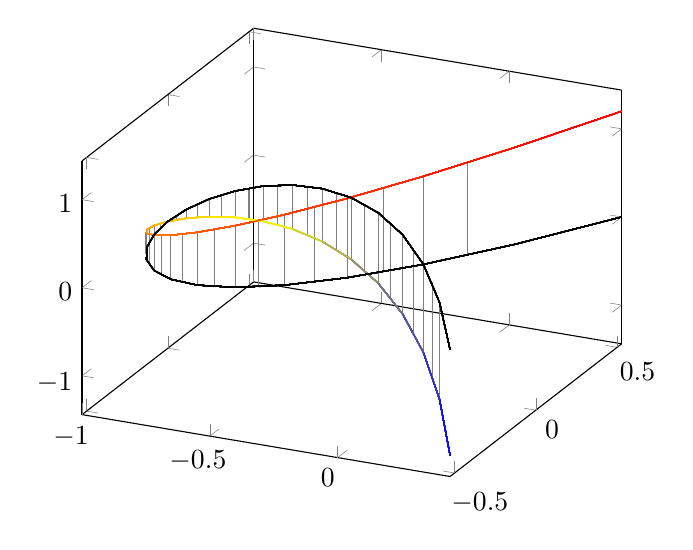
\begin{tikzpicture}
\begin{axis}
    \pgfplotsinvokeforeach{-1.1, -1.05, ..., 1.1}
    { \draw[gray] (#1*#1-1,#1*#1*#1-#1,#1) -- (#1*#1-1,#1*#1*#1-#1,0);
    }
    \addplot3[variable=t,mesh,domain=-1.2:1.2] (t^2-1,{t*(t^2 - 1)}, t);
    \addplot3[variable=t,mesh,domain=-1.2:1.2,color=black] (t^2-1,{t*(t^2 - 1)}, 0);
\end{axis}
\end{tikzpicture}
\end{center}

Another example is the curve with a \emph{cusp}: $X': y^2 = x^3$, singularity at $(0, 0)$.
We can normalize the ring $R = k[x, y] / (y^2 - x^3)$ similarly as $\widetilde{R} = k[x, y, t] / (y^2 - x^3, t^2 -x, y - tx)$ (taking $t = y/x$), which corresponds to the curve $X = \{(x, y, t): y^2 = x^3, t^2 = x, y = tx\} = \{(t^2, t^3, t)\}$.
It's Jacobian is given by
$$
J = \begin{pmatrix}
    -3x^2 & -2y & 0 \\ 1 & 0 & -2t \\ -t & 1 & -x
\end{pmatrix}
$$
whose determinant is 0 and the first two columns are linearly independent, so has rank $2 = 3 - 1$.
In fact, we have $X = \{(t^2, t^3, t)\} \simeq \bA^1$.

\begin{center}
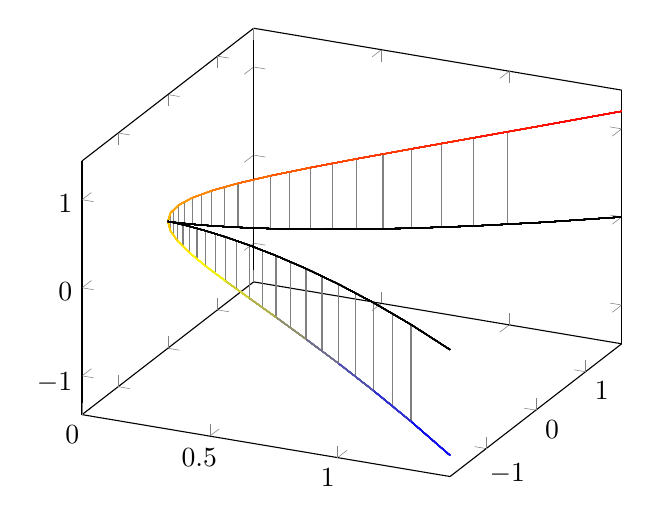
\begin{tikzpicture}
\begin{axis}
    \pgfplotsinvokeforeach{-1.1, -1.05, ..., 1.1}
    { \draw[gray] (#1*#1,#1*#1*#1,#1) -- (#1*#1,#1*#1*#1,0);
    }
    \addplot3[variable=t,mesh,domain=-1.2:1.2] (t^2,t^3,t);
    \addplot3[variable=t,mesh,domain=-1.2:1.2,color=black] (t^2,t^3,0);
\end{axis}
\end{tikzpicture}
\end{center}

We denote as $\frc$ for the annihilator of $\scO / \scO'$, call it as the \emph{conductor} of $\scO$ into $\scO'$.
It is a coherent sheaf of ideals on $X'$ and its variety $S'$ is a set of points on $X'$ which are not normal.
Put $S = p^{-1}(S')$, so that $p$ gives an isomorphism between $X \backslash S$ and $X' \backslash S'$, i.e. $p$ is a birational morphism.
For $Q \in X'$, $\frc_Q = \{f \in \scO_Q': fg \in \scO_Q' \,\forall g \in \scO_Q\}$, which is also the largest ideal of $\scO_Q'$ that is also an ideal of $\scO_Q$.
We have a chain of inclusions
$$
\scO_Q \supset k + \frr_Q \supset \scO_Q' \supset k + \frc_Q
$$
where $\frr_Q$ is the radical of $\scO_Q$, same as the set of $f \in \scO_Q$ such that $f(P) = 0$ for all $P \mapsto Q$.

\subsection{Case of an algebraic curve}

In case of curves, a curve is normal if and only if nonsingular, so normalization corresponds to \emph{desingularization} for curves.
For a normalization $p: X \to X'$, the corresponding $S' \subset X'$ and $S = p^{-1}(S') \subset X$ are finite sets, and especially, $S'$ is nothing but the set of singular points of $X'$.
For all $Q \in X'$, $\delta_Q := \dim(\scO_Q / \scO'_Q)$ is finite, and positive if and only if $Q \in S'$.
$\delta_Q$ is also an \emph{analytic invariant}: it is preserved under taking completions: $\delta_Q = \dim (\widehat{\scO_Q} / \widehat{\scO_Q'})$.
We call that two singular points are \emph{analytically isomorphic} if they have same $\delta_Q$.

We know that $\scO_Q / \scO_Q'$, $\scO_Q' / \frc_Q$, and $\scO_Q / \frc_Q$ are all finite dimensional, so $\frc_Q \supset \frr_Q^n$ for some $n > 0$ and we get 
\begin{equation}
\label{eqn:rad}
    k + \frr_Q \supset \scO_Q' \supset k + \frr_Q^n.
\end{equation}

\begin{question}
For given $X'$ and $Q \in X'$, how can we compute $\delta_Q$?
\end{question}

\subsection{Construction of a singular curve from its normalization}

We can also ``denormalize'' a nonsingular curve $X$, i.e. do opposite direction of above.
More precisely, let $X$ be an irreducible nonsingular curve and $S \subset X$ be a finite set.
Let $R$ be an equivalence relation on $S$, and define $S' := S / R$.
Then Proposition 2 says that $X' := (X \backslash S) \cup S'$ with the canonical projection $p:X \to X'$ becomes an algebraic curve with singularities at $S'$.
Intuitively, we are identifying points in $S$ under the equivalence relation $R$ to get a singular curve $X'$ with singular points $S'$.

Here's a sketch of the ``construction'' of $\scO'$, the structure sheaf of $X'$.
Put $\scO_Q := \cap_{P \to Q} \scO_P$ (taking intersection) and $\frr_Q$ to be the radical of $\scO_Q$.
For each $Q \in S'$, choose $\scO_Q' \subset \scO_Q$ different from $\scO_Q$ so that \eqref{eqn:rad} is satisfied for some $n$.
For $Q \in X' \backslash S'$, define $\scO_Q' = \scO_Q$.
Then this will form a sheaf $\scO'$.

To prove that $(X, \scO_X)$ is a normalization of $(X', \scO')$, it is enough to check when $X$ is affine.
Assume that $A$ is a coordinate ring of $X$.
Let $A' = \cap_{Q \in X'} \scO_Q' \subset A$.
For each $P \in X$, let $\fra_P = \{f \in A: f(P) = 0\} \subset A$ be the maximal ideal corresponds to $P$ and $\frr = \cap_{P \in S} \fra_P$.
By \eqref{eqn:rad} there exists $n$ such that $A' \supset k + \frr^n$, and one can show that $A$ is an $A'$-module of finite type; so is integral over $A'$.
Then $A'$ is also a $k$-algebra of finite type and we have a corresponding affine variety $Y$, and $X$ becomes a normalization of $Y$ ($A$ is an integral closure of $A'$).
Now we can prove that $Y$ is actually isomorphic to $(X', \scO')$.

% (CJ, Connor): In affine case, it should work in this way: for $X = \Spec A, Y = \Spec B$ affine with common closed subscheme $Z = \Spec C$, then identifying $X$ and $Y$ along $Z$ corresponds to
% \begin{center}
%     \begin{tikzcd}
%         A \times_C B \arrow[r] \arrow[d] & B \arrow[d, twoheadrightarrow] \\
%         A \arrow[r, twoheadrightarrow] & C
%     \end{tikzcd}
% \end{center}

The above proof is constructive, i.e. it gives a coordinate ring $A'$ of a corresponding $X'$ when $X = \Spec A$ is affine.
Here's a different approach that might be easier to understand, at least for me.
Consider the case when $X = \bA^1 = \Spec k[x]$ and $S = \{1, -1\}$, so that we are identifying two points on a line to get a singular curve.
Then the resulting $X' = X / \{1 \sim -1\} = \Spec A'$ should correspond to a universal object to the following diagram
\begin{center}
    \begin{tikzcd}
        & \{1\} \arrow[d, hookrightarrow] \arrow[rdd, bend left] & \\
        \{-1\} \arrow[r, hookrightarrow] \arrow[rrd, bend right] & \bA^1 \arrow[rd, twoheadrightarrow] & \\
        & & X'
    \end{tikzcd}
\end{center}
which corresponds to the diagram of rings
\begin{center}
    \begin{tikzcd}
        & k & \\
        k & k[t] \arrow[l, "\ev_{-1}"] \arrow[u, "\ev_{1}"] & \\
        & & A' \arrow[lu, hookrightarrow] \arrow[llu, bend left] \arrow[luu, bend right]
    \end{tikzcd}
\end{center}
In other words, $A'$ is a subring $A' = \{f \in k[t]: f(-1) = f(1)\}$.
One can show that $A'$ is generated by two elements $t^2 - 1$ and $t^3 - t$, i.e. $A' = k[t^2 - 1, t^3 - t]$, and $A'$ is not integrally closed since $t = \frac{t^3 - t}{t^2 - 1}$ is in its fractional field, and integral over $A'$ ($t^2 = (t^2 - 1) + 1$), but $x \not \in A'$. We also know that $A'[t] = k[t] = A$, so $A$ is an integral closure of $A'$.
Now, one can prove that $A' \simeq k[x, y] / (y^2 - x^3 - x^2)$ via $(t^2 - 1, t^3 - t) \leftrightarrow (x, y)$.

Here's a slightly more complicated example: $X = k[s, t] / (s^2 + t^2 - 1)$ and $S = \{(0, -1), (0, 1)\}$, i.e. identifying two points on a circle.
Let $B' = \{f \in k[s, t]: f(0, -1) = f(0, 1)\}$ and $A' = B' / (s^2 + t^2 - 1)$.
One can show that $B' = k[t^2 - 1, t(t^2 - 1), s, st]$, hence
$$
A' = k[-s^2, -s^2 t, s, st] / (s^2 + t^2 - 1) = k[s, st] / (s^2 + t^2 - 1).
$$
and this is isomorphic to $k[x, y] / (y^2 - x^2 (1 - x^2))$ under the map $(s, st) \leftrightarrow (x, y)$.
This gives an equation $y^2 = x^2 (1 - x^2)$ of $X'$.

\begin{center}
\begin{tikzpicture}[scale=1.5]
  \tkzInit[xmin=-2,xmax=2,xstep=1,ymin=-2,ymax=2,ystep=1]
  % \tkzGrid[sub]
  \tkzAxeX[step=1]
  \tkzAxeY[step=1]
  \tkzFctPar[samples=400,domain=-pi:pi]{cos(t)}{cos(t) * sin(t)}
\end{tikzpicture}
\end{center}

Another examples is when we identify three distinct points.
Consider $X = \bA^1$ and $S = \{-1, 0, 1\}$.
By the above arguments, $X' = X / S = \Spec A'$ where $A' = \{f \in k[t]: f(-1) = f(0) = f(1)\}$.
One can show that
$$
A' = k[t(t^2 - 1), t^2(t^2 - 1), t^3(t^2 - 1)] \simeq k[x, y, z] / (y^2 - xz, x^4 - y(y^2 - x^2)),
$$
i.e. $X'$ is an intersection of two surfaces $y^2 = xz$ and $x^4 = y(y^2 - x^2)$ in $\bA^3$.

\begin{center}
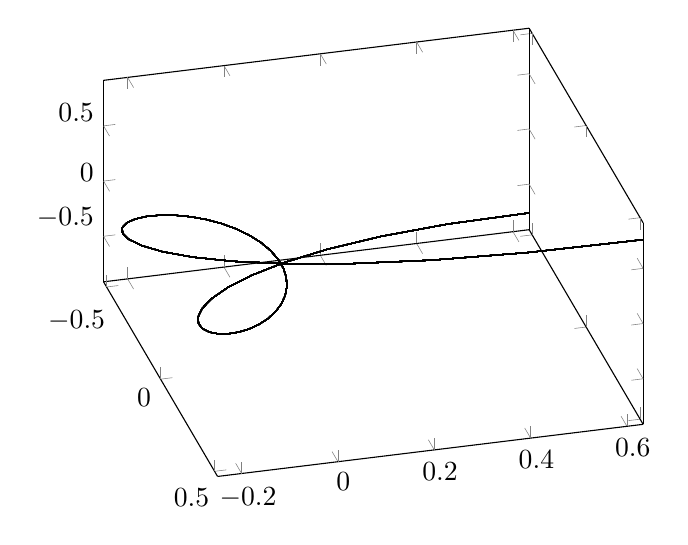
\begin{tikzpicture}
\begin{axis}[view={75}{45}]
    % \pgfplotsinvokeforeach{-1.1, -1.05, ..., 1.1}
    % { \draw[gray] (#1*#1-1,#1*#1*#1-#1,#1) -- (#1*#1-1,#1*#1*#1-#1,0);
    % }
    % \addplot3 [
    %     surf,
    %     shader=faceted,
    %     fill opacity=0.75,
    %     samples=25,
    %     domain=-4:4,
    %     y domain=-4:4,
    %     on layer=foreground,
    % ] {x^2-y^2};
    % \addplot3[
    %     surf,
    %     domain=-1.2,1.2,
    %     samples=100,
    %     samples y=11,z buffer=sort
    % ]
    % ({y*sin(deg(x))},
    % {y*cos(deg(x))},
    % {x});
    \addplot3[variable=t,mesh,domain=-1.2:1.2,samples=50,color=black] (t^3-t,t^4-t^2,t^5-t^3);
    % \addplot3[variable=t,mesh,domain=-1.2:1.2,color=black] (t^2-1,{t*(t^2 - 1)}, 0);
\end{axis}
\end{tikzpicture}
\end{center}



\subsection{Singular curve defined by a modulus}

Using the previous construction, we can define a (singular) curve $X_\frm$ from a modulus $\frm$ of $X$.
Here we assume $\deg(\frm) \ge 2$ (otherwise $X_\frm = X$).
Let $S$ be the support of $\frm$.
Take $S' = \{Q\}$ to be a single point and $X' := (X \backslash S) \cup S'$ (i.e. merge every singular points of $X$ into a single point).
Put
\begin{align*}
    \frc_Q &:= \{f \in \scO_Q : f \equiv 0\,(\mathrm{mod}\,\frm)\} \\
    \scO_Q' &:= k + \frc_Q
\end{align*}
Then we can apply the previous construction to get a singular curve $X_\frm$ with a unique singular point $Q$, where
$$
\delta_Q = \dim (\scO_Q /\scO_Q') = \dim (\scO_Q / (k + \frc_Q)) = \dim (\scO_Q / \frc_Q) - 1 = \deg(\frm) - 1.
$$
For example, when $\frm = 2P$ for some $P \in X$, the corresponding $X_\frm$ with $p:X \to X_\frm$ has an \emph{ordinary cusp} at $Q = p(P)$, i.e. analytically isomorphic to $y^2 - x^3$ at $Q$.
When $\frm = P_1 + P_2$ with $P_1 \ne P_2$, it identifies two different points on $X$, and the resulting curve $X_\frm$ is analytically isomorphic to $xy = 0$ at the singular point $Q$ (i.e. $Q$ is a \emph{node}).

\begin{question}
For a given irreducible nonsingular curve $X$ (in terms of certain set of equations) and a modulus $\frm$, how to compute $X_\frm$, i.e. how to find a corresponding equation of $X_\frm$?
Can we do this at least for $X = \bP^1$ or $\bA^1$?
\end{question}


\section{Riemann--Roch theorems}

\subsection{Notations}

Now assume $X$ (and so $X'$) are complete curves, so also projective.
Let $g$ be the genus of $X$ and put
\begin{align*}
    \delta &= \sum_{Q\in S'} \delta_Q \\
    \pi &= \delta + g.
\end{align*}
For a divisor $D$ on $X$ prime to $S$, we have a sheaf $\cL(D)$ on $X$ associated to it.
Under the birational map $X \to X'$, we can define a sheaf $\cL'(D)$ on $X'$ via
$$
\cL'(D)_Q := \begin{cases} \cL(D)_Q & Q \not \in S' \\ \scO_Q' & Q \in S'. \end{cases}
$$
Also, we define
\begin{align*}
    L'(D) = \rH^0(X', \cL'(D)), &\quad I'(D) = \rH^1(X', \cL'(D)),\\
    l'(D) = \dim L'(D), &\quad i'(D) = \dim I'(D)
\end{align*}
as in the nonsingular case.
Especially, when $X' = X_\frm$, we denote above as $L_\frm(D), I_\frm(D), l_\frm(D), i_\frm(D)$.


\subsection{The Riemann--Roch theorem (first form)}

The Riemann--Roch theorem for singular curves has a same form as nonsingular case, but just replace $l(D), i(D), g$ with $l'(D), i'(D), \pi$: for any divisor $D$ prime to $S$,
$$
    l'(D) - i'(D) = \deg(D) + 1 - \pi.
$$
We can prove it by using the same argument as in Chapter 2 for nonsingular curves: by considering a cohomology sequence, on can reduce it to the case of $D = 0$, i.e. $\chi(X', \scO') = 1 - \pi$.
Using $0 \to \scO' \to \scO \to \scO / \scO' \to 0$ and $\chi(X', \scO / \scO') = \dim \rH^0(X', \scO / \scO') = \delta$ ($\scO / \scO'$ is supported on $S'$), it reduces to prove that $\chi(X', \scO) = 1 - g$.
This follows from the fact that $\rH^q(X, \scO_X) = \rH^q(X', \scO)$ for all $q \ge 0$: this holds essentially because $X \to X'$ is a finite map.


\subsection{Application to the computation of the genus of an algebraic curve}

By considering $D = 0$, we get $\pi = i'(0) = \dim \rH^1(X', \scO')$.
As a corollary, we can compute \emph{arithmetic genus} $p_a(X')$ of a curve: recall that it is defined as
$$
p_a(X') = 1 - \chi(X') = 1 - \dim \rH^0(X', \scO') + \dim \rH^1(X', \scO')
$$
Since $X'$ is connected, $\dim \rH^0(X', \scO') = 1$ and we get
$$
p_a(X') = \pi = \delta + g.
$$
Note that $p_a(X')$ depends on the base field $k$; see also \href{https://stacks.math.columbia.edu/tag/0BY6}{Stacks project} (but again, we assume $k$ is algebraically closed).
This is useful since $p_a(X')$ and $\delta$ are supposed to be easy to compute, and we can use them to compute $g$.
For example, if $X'$ is a complete intersection of $r-1$ hypersurfaces of degre $a_1, \dots, a_{r-1}$ in $\bP^{r}$ we get
$$
\pi = \frac{1}{2} a_1 \cdots a_{r-1}\left(\sum_{i=1}^{r-1} a_i - r - 1 \right) + 1
$$
and when $r = 2$, we get a \emph{Pl\"ucker formula}
$$
g = \frac{1}{2} d (d - 3) + 1 - \delta.
$$

\subsection{Genus of a curve on a surface}

Let $V$ be a projective non-singular surface and $X' \subset V$ be a curve in it.
Then we have a general formula for $p_a(X')$ in terms of a certain intersection number:
$$
p_a(X') = 1 + \frac{1}{2}X'\cdot(X' + K)
$$
where $K$ is a canonical divisor of $V$, i.e. divisor of a non-zero differential form of degree 2.


\section{Differentials on a singular curve}


\subsection{Regular differentials on $X'$}

A differential $\omega$ on $X$ is said to be \emph{regular at $Q \in S'$} if $\sum_{P \to Q} \Res_P(f\omega) = 0$ for all $f \in \scO_Q'$.
We denote $\underline{\Omega}_Q'$ for the set of regular differentials, which is a $\scO_Q'$-submodule of $D_k(X)$.
If we put
$$
\underline{\Omega}_Q := \bigcup_{P \to Q} \underline{\Omega}_P,
$$
then $\underline{\Omega}_Q \subset \underline{\Omega}_Q'$ and we have a duality between $\scO_Q / \scO_Q'$ and $\underline{\Omega}_Q' / \underline{\Omega}_Q$, given by the pairing $(f, \omega) \mapsto \sum_{P \to Q} \Res(f\omega)$ above.
When $X' = X_{\frm}$ with $\frm = \sum_P n_P P$, $\omega$ is regular on $X'$ if and only if
$$
\sum_{P \in S} \Res_P(\omega) = 0 \quad\text{and}\quad v_P(\omega) \ge -n_P\,\forall P \in S.
$$
For general case, regular differentials are characterized as follows: $\omega$ is everywhere regular on $X'$ if and only if $\Tr_g(\omega) = 0$ for every rational function $g$ on $X$ which is not a $p$-th power (if $\cha (k) = p$) and which belongs to all $\scO_Q'$, $Q \in S'$.


\subsection{Duality theorem}

Serre duality also extends to singular curves.
For a divisor $D$ prime to $S$, associate a sheaf $\underline{\Omega}'(D)$ by
$$
\underline{\Omega}'(D)_Q = \begin{cases}
    \underline{\Omega}_Q' & Q \in S' \\ \underline{\Omega}(D)_Q & Q \not \in S'.
\end{cases}
$$
We also put $\Omega'(D) = \rH^0(X', \underline{\Omega}'(D))$.
Then $\omega \in \Omega'(D)$ if and only if it is regular at all $Q \in S'$ and also $v_P(\omega) \ge v_P(D)$ for all $P \not \in S$.
Then we have $\Omega'(D) \simeq I'(D)^\ast = \rH^1(X', \cL'(D))^\ast$, and we get $i'(D) = \dim \Omega'(D)$.
Especially, $i'(0) = \dim\Omega'(0) = \pi$, i.e. the dimension of everywhere regular differential forms on $X'$ is $\pi$.
Proof uses the ad\`elic language in Chapter 2.


\subsection{The equality $n_Q = 2 \delta_Q$}

For $Q \in S'$, we can identify the conductor ideal $\frc_Q$ with a divisor $\sum_{P \to Q} n_P P$ such that $\frc_Q = \{f \in \scO_Q: (f) \ge \sum_{P \to Q} n_P P\}$.
By using the duality between $\scO_Q / \scO_Q'$ and $\underline{\Omega}_Q' / \underline{\Omega}_Q$, one can see that they have the same annihilators and $f \in \frc_Q$ iff $v_P(f \omega) \ge 0$ for all $P \to Q$ and $\omega \in \underline{\Omega}_Q'$.
In other words, $n_P = \sup_{\omega \in \underline{\Omega}_Q'} (- v_P(\omega))$.
Now put $n_Q := \sum_{P \to Q} n_P$ be the degree of the divisor $\frc_Q$.
Then we have an inequality between $n_Q$ and $\delta_Q$:
$$
\delta_Q + 1 \le n_Q \le 2 \delta_Q
$$
for all $Q \in S'$, and $n_Q = 2 \delta_Q$ if and only if $\underline{\Omega}_Q'$ is a free $\scO_Q'$-module of rank 1.
When this holds for all $Q \in S'$, $\underline{\Omega}'$ is locally free and corresponds to a class of divisors of $K'$ on $X'$, where $K = K' - \frc$.
Taking $\deg$ gives $\deg(K') = 2\pi - 2$, and $\underline{\Omega}'(D) \simeq \cL'(K' - D)$, which gives a definitive form of the Riemann--Roch theorem
$$
l'(D) - l'(K' - D) = \deg(D) + 1 - \pi.
$$

For the previous examples of $\frm = P_1 + P_2$ or $\frm = 2P$, the theorem shows that $\delta_Q = 1$ for $Q \in X_\frm$, since $n_Q = 2$ and $1 = \frac{n_Q}{2} \le \delta_Q \le n_Q - 1 = 1$ for both cases.

\subsection{Complements}

Note that $n_Q = 2 \delta_Q$ holds when
\begin{itemize}
    \item $X'$ is a complete intersection in a projective space,
    \item $X'$ is embedded in a nonsingular surface $V$.
\end{itemize}
% In other words, if $n_Q$ is odd, then $X' = X_\frm$ is neither be a complete intersection nor embedded in a nonsingular surface.

% --- Bibliography ---

% Start a bibliography with one item.
% Citation example: "\cite{williams}".

% \bibliographystyle{acm} % We choose the "plain" reference style
% \bibliography{refs} % Entries are in the refs.bib file


% \begin{thebibliography}{1}

% \bibitem{williams}
%    Williams, David.
%    \textit{Probability with Martingales}.
%    Cambridge University Press, 1991.
%    Print.

% % Uncomment the following lines to include a webpage
% % \bibitem{webpage1}
% %   LastName, FirstName. ``Webpage Title''.
% %   WebsiteName, OrganizationName.
% %   Online; accessed Month Date, Year.\\
% %   \texttt{www.URLhere.com}

% \end{thebibliography}

% --- Document ends here ---

\end{document}